\documentclass[12pt,a4paper,titlepage]{article}
\usepackage{graphicx}

\title{COP290: Design Practices\break\\User Registration App}
\author{Akshit Tyagi (2014EE10710) \\ Rishabh Kumar (2014PH10817) \\ Karan Dwivedi (2014CS10227) }
\date{15 January 2016}
\begin{document}
\maketitle

`User Registration App' is a simple Android app to test communication with a server using Volley JSON library. It takes in the names and entry numbers of team members through its user friendly GUI and sends it to the server when Submit button is pressed. We also check if the user types invalid (or blank) input.

The app also recieves the server response and shows it to the user. In case the server sent a ``Registration failed'' message, the app prompts the user to try again later.

\section{User Interface}

\begin{figure}[!ht]
	\centering
	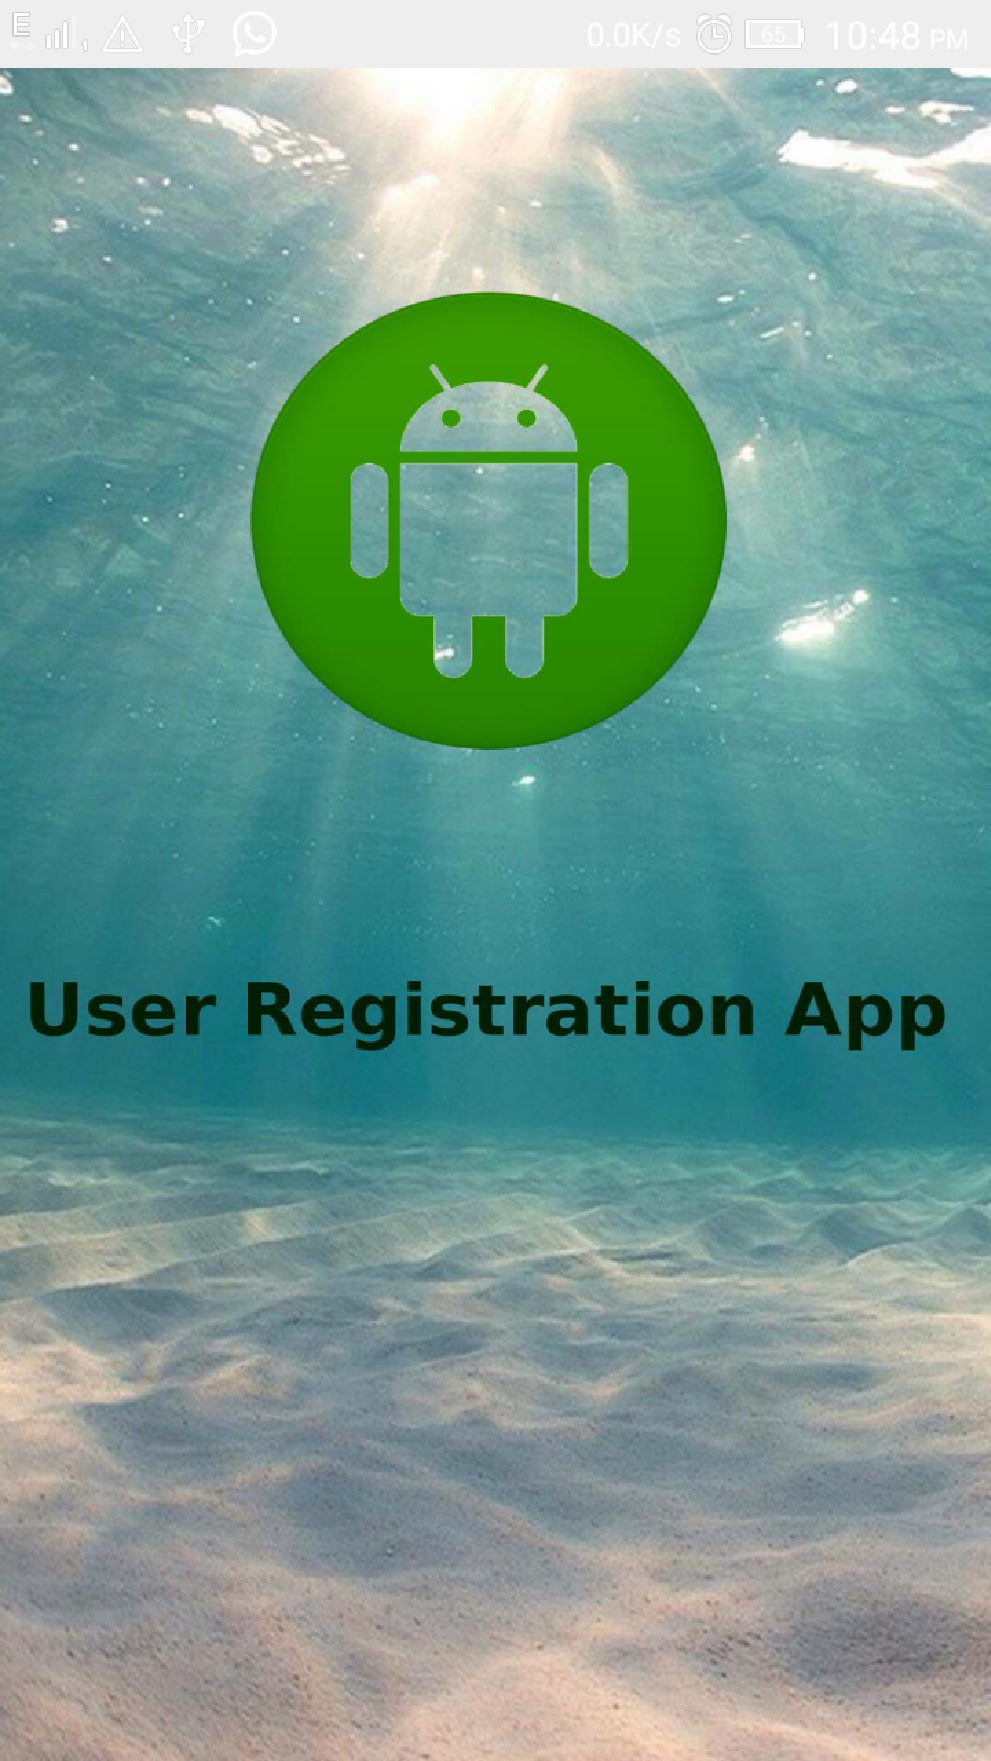
\includegraphics[width=0.5\textwidth]{./UserInterface}
	\caption{Primary Screen}
\end{figure}



\begin{itemize}
	\item Details of the screens visible to the user
	\item[] The app has only one activity which is visible to the user. The activity has 6 input fields and a floating submit button. To register on the web server, the user enters the input using inbuilt keyboard and taps the submit button. In case there is an error in the input or the server response, the user in prompted via a Toast.
	      
	\item Animations, buttons (enabled/disabled under what conditions)
	\item[] Following Google's material design principles, the screen has a floating submit button, which connects to the server only after the user has entered valid input in all fields. Otherwise, it highlights the incorrect inputs and prompts the user to correct them.
	\item Actions performed when a user enters information, presses a button/icon etc.
	\item[] When the user taps any input field, the keyboard shows. 
	\item[] If the user leaves an input field without entering valid data, the field is highlighted.
	\item[] On pressing the submit button, the app checks the input and if found valid, sends it to the web server and recieves its response.
\end{itemize}

\section{Implementation Details}

\begin{itemize}
	\item Organization of user information (Is it in a special User class, or is it distributed in arrays for each user entry)
	\item[] Data
	\item[] JSON Object
	\item Methods to verify the user information: Highlight the errors handled by the code
	\item[] Once on leaving the input field
	\item[] Once on pressing the submit button
	\item  High	level functions/methods used and descriptions of each one	
	\item [] sending
	\item[] recieving
	\item[] oncreate
	\item Methods for network communication. You can cite material that you used to create the application~\cite{android_network_tutorial}.
\end{itemize}


\section{Error Handling}
\begin{itemize}
	        
	\item error scenarios and handling method
	      
	      
	\item How to make sure that the user is entering a valid entry number
	\item How to make sure that the user is entering a valid name
	          
	\item – E.g.	user	is	asked	for	Entry	number	but	gives	an	invalid	one	
\end{itemize}

The code for the project is being maintained in this repository: {\em https://prathmesh\_kallurkar@bitbucket.org/prathmesh\_kallurkar/user-registration-app.git}.

\bibliographystyle{abbrv}
\bibliography{references}

\end{document}
